\begin{frame}{Praktische Analyse}{Programmierfehler}
    Overflow-anfällig sind Sprachen, welche direkte Zugriffe auf die Speicherstrukturen\\ des Systems ermöglichen:
    \begin{itemize}
        \vspace{1em}
        \item Assembly
        \item C/C++
        \item Fortran
    \end{itemize}
\end{frame}

\begin{frame}{Praktische Analyse}{Programmierfehler}
    Problematisch sind Funktionen, welche
    keine Kontrolle auf die Länge des Inputs implementieren: %ausüben / durchführen
    \begin{itemize}
        \vspace{1em}
        \item \codeline{gets(buffer)}\\ Erwartet Input und kopiert diesen in den angegebenen Speicher
        \vspace{1em}
        \item \codeline{strcopy(buffer, input)}\\ Kopiert einen Input
        in den angegebenen Speicher
    \end{itemize}
\end{frame}


\begin{frame}{Praktische Analyse}{Format-String-Schwachstelle}
    Unvorsichtige Verwendung von Formatierungsfunktionen:
    \begin{itemize}
        \vspace{1em}
        \item \codeline{printf(``\%s'', chars)}\\ Korrekte/Sichere Verwendung
        \vspace{1em}
        \item \codeline{printf(chars)}\\ Falsche/Unsichere Verwendung
    \end{itemize}
%BIG CODEIMAGE
\end{frame}

\begin{frame}{Praktische Analyse}{Demonstration}
    \begin{figure}[h]
        \centering
        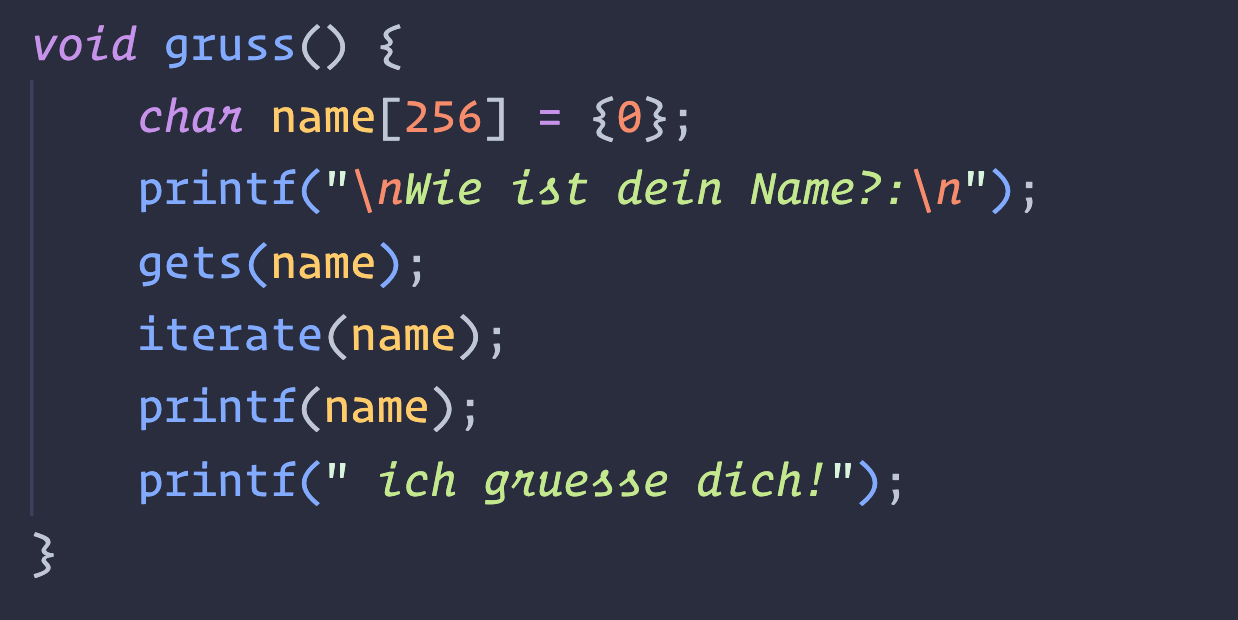
\includegraphics[width=0.7\textwidth,height=0.75\textheight,keepaspectratio]{images/gruss.png}
        \caption{Funktion \codeline{gruss()} }
    \end{figure}
\end{frame}

\begin{frame}{Praktische Analyse}{Demonstration}
    \begin{figure}[h]
        \centering
        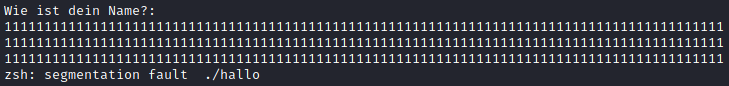
\includegraphics[width=0.7\textwidth,height=0.75\textheight,keepaspectratio]{images/segfault.png}
        \caption{Segmentierungsfehler}
    \end{figure}
    \begin{figure}[h]
        \centering
        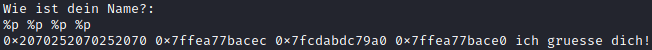
\includegraphics[width=0.7\textwidth,height=0.75\textheight,keepaspectratio]{images/adressen.png}
        \caption{Ausgegebene Speicheradressen}
    \end{figure}
\end{frame}

\begin{frame}{Praktische Analyse}{Demonstration}
    \begin{figure}[h]
        \centering
        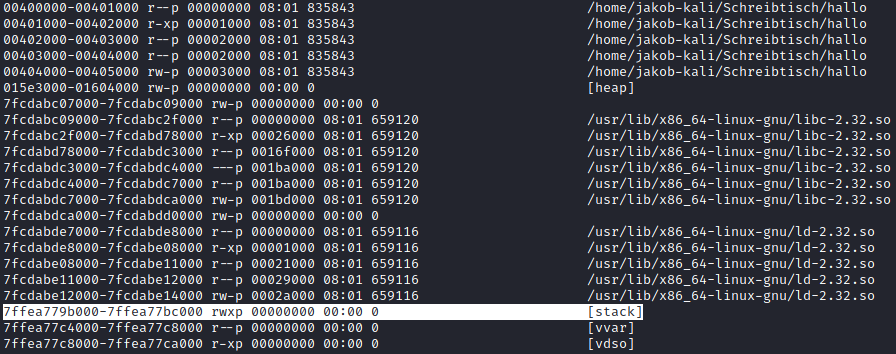
\includegraphics[width=0.7\textwidth,height=0.75\textheight,keepaspectratio]{images/map.png}
        \caption{Memory Map}
    \end{figure}
    \begin{figure}[h]
        \centering
        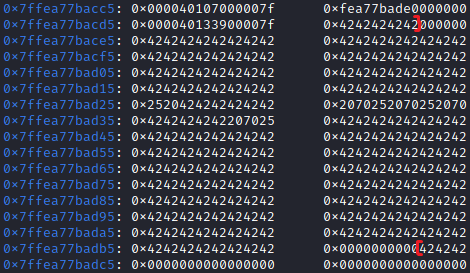
\includegraphics[width=0.7\textwidth,height=0.75\textheight,keepaspectratio]{images/buffer.png}
        \caption{Speicherinhalt}
    \end{figure}
\end{frame}

\begin{frame}{Praktische Analyse}{Demonstration}
    \begin{figure}[h]
        \centering
        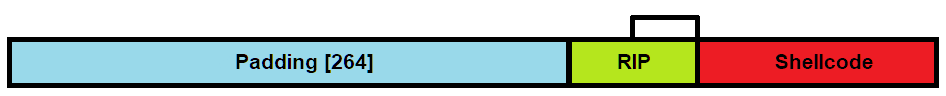
\includegraphics[width=0.7\textwidth,height=0.75\textheight,keepaspectratio]{images/payload1.png}
        \caption{Payload 1}
    \end{figure}
    \begin{figure}[h]
        \centering
        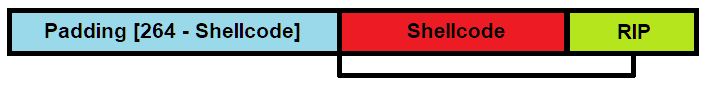
\includegraphics[width=0.7\textwidth,height=0.75\textheight,keepaspectratio]{images/payload2.png}
        \caption{Payload 2}
    \end{figure}
    \begin{figure}[h]
        \centering
        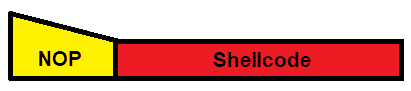
\includegraphics[width=0.7\textwidth,height=0.75\textheight,keepaspectratio]{images/nop.png}
        \caption{NOP Slide}
    \end{figure}
\end{frame}

\begin{frame}{Praktische Analyse}{Demonstration}
    \begin{figure}[h]
        \centering
        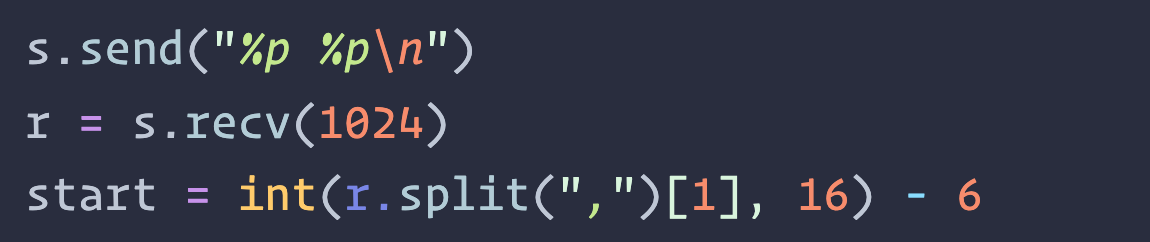
\includegraphics[width=0.7\textwidth,height=0.75\textheight,keepaspectratio]{images/format.png}
        \caption{Format-String-Ausgabe}
    \end{figure}
    \begin{figure}[h]
        \centering
        
\includegraphics[width=0.7\textwidth,height=0.75\textheight,keepaspectratio]{images/rip.png}
        \caption{RIP}
    \end{figure}
    \begin{figure}[h]
        \centering
        
\includegraphics[width=0.7\textwidth,height=0.75\textheight,keepaspectratio]{images/payload.png}
        \caption{Payload}
    \end{figure}
\end{frame}

\begin{frame}{Praktische Analyse}{Demonstration}
    \begin{figure}[h]
        \centering
        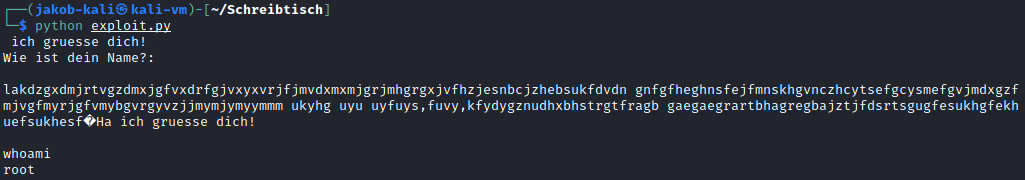
\includegraphics[width=0.7\textwidth,height=0.75\textheight,keepaspectratio]{images/root.png}
        \caption{Root Shell}
    \end{figure}
\end{frame}

